\chapter{ИНСТРУМЕНТАЛЬНЫЕ СТРЕДСТВА РАЗРАБОТКИ сайта}

\section{Обоснование создания системы}
В настоящее время продавцам на маркетплейсах в связи со стремительным развитием конкуренции нужно правильно распределять свой бюджет, рассчитывать юнит- экономику для своих товаров, уметь получать данные о своих продажах, поступлениях, расходах и т.д. Однако эти данные предоставляются в сырых слабоструктурированных файлах (csv, xlsx), которые требуют долгой обработки, сложны для понимания начинающим продавцам, а также отнимают много времени и сил, которые могли бы пойти на иные бизнес-процессы ~\cite{problemSellers}.

Альтернативные подходы к обработкам информации на маркетплейсах сопутствуют либо дорогостоящими подписками на сервисы аналитики, либо трудоемкой работой в процессорных редакторах вручную, либо изучение сложных готовых программ по автоматизации бизнес-процессов.

При покупке подписки на сервисы аналитики продавец будет пользоваться сервисом, в котором функционал может не соответствует требуемым предпочтениям. Пока пользователь найдет сервис с набором инструментов, который в полной мере будет удовлетворять потребностям его бизнеса, пройдет довольно много времени и средств, будут куплены подписки на сервисы, что ведет к финансовым издержкам.

Один из вариантов – корпоративные системы управления отчетности 1С, при использовании которого возникают следующие особенности~\cite{integracia1C}:
\begin{itemize}
 \item Финансовые затраты на лицензию~\cite{integracia1C};
 \item Доработка системы под свои нужны ~\cite{integracia1C};
 \item Ограниченность функционала 1С для работы с маркетплейсами~\cite{integracia1C}.
\end{itemize}

Интеграция с маркетплейсами требуют специализированных знаний ~\cite{integracia1C}, платных модулей, либо постоянный найм программистов для поддержки связи 1С и маркетплейсов~\cite{integracia1C}. 

Из вышеперечисленного следует, что для малого и среднего бизнеса такой подход не является рациональным в плане финансовых и трудовых затрат. Помимо этого, каждый маркетплейс имеет свои виды выходных данных, отчетов и подключений, а разрабатывать под каждый маркетплейс свою систему в 1С просто не имеет смысла, особенно в плане финансовых затрат.

Альтернативой специализированным системам являются универсальные табличные процессоры, имеющие легкий функционал и не требующие углубленных навыков и финансовых затрат для начала работы с ними. Но несмотря на широкую доступность и легкость освоения этих сервисов, трудовые затраты на занесения данных в таблицы и их последующая обработка занимает слишком много времени для регулярного анализа. Такой ручной метод подходит для продавцов, у которых небольшие продажи.

Таким образом, проблема отсутствия специализированного, общедоступного, легкого и интуитивно понятного инструмента, который закрывал бы потребности продавцов и облегчал им жизнь, стоит довольно остро.

Из всего вышесказанного требуется разработать веб – инструмент, который обладает следующими характеристиками:

\begin{itemize}
 \item Доступность;
 \item Кроссплатформенность;
 \item Ограниченность функционала 1С для работы с маркетплейсами~\cite{integracia1C}.
 \item Универсальность под изменения маркетплейсов;
 \item Приятный глазу пользовательский интерфейс.
\end{itemize}

Из всего перечисленного было решено создать интерактивный сайт, который:
\begin{itemize}
 \item  Является общедоступным и недорогим в производстве;
 \item  Запускается на любом устройстве с выходом в интернет;
 \item  Имеет продуманную логику;
 \item  Имеет регистрацию и авторизацию;
 \item  Легко изменяется под обновления маркетплейсов;
 \item  Имеет приятный и интуитивно понятный интерфейс.
\end{itemize}

\section{Основа технических инструментов разработки сайта}

Для реализации автоматизации веб – приложения и его функциональных и технических требований необходимо составить набор технологий, на которых будет строиться веб – приложение. Архитектура сайта будет строиться на таких компонентах, как:

\begin{enumerate}
     \item Язык разметки (HTML) – Используется для создания семантической структуры веб – приложения, а точнее каждой страницы веб приложения~\cite{webProgramming};
     \item Язык стилей (CSS) – Используется для управления визуальным составляющим сайта~\cite{webProgramming};
     \item Язык программирования – Служит для реализации динамического поведения веб – страниц, логики веб – приложений и взаимодействия сайта с внешними ресурсами. Основными языками программирования для создания сайтов служат языки: C++, Python, JavaScript и TypeScript~\cite{webProgramming};
     \item API методы и запросы, с помощью которых получаются данные с сайтов~\cite{usingAPI1}. Это набор правил и протоколов, позволяющих различным программным компонентам обмениваться данными. В рамках данного проекта API-запросы используются для получения отчётов о продажах и остатках с маркетплейсов Ozon и Wildberries. Запросы отправляются по протоколу HTTPS с использованием методов GET и POST, а полученные данные обрабатываются в форматах JSON, CSV и XLSX;
     \item Фреймворк для построения полноценного веб-приложения – необходим для создания современного веб-приложения, объединяющего клиентскую и серверную части. Фреймворк должен поддерживать серверный рендеринг для ускорения загрузки страниц, статическую генерацию для контента, который редко меняется, и маршрутизацию на основе файловой структуры. Встроенная поддержка API-роутов позволяет создавать серверные компоненты в рамках одного проекта, что упрощает разработку и развёртывание. Высокая производительность и оптимизация загрузки страниц критически важны для пользовательского опыта;
     \item База данных – необходима для постоянного хранения учётных записей пользователей (логины, хеши паролей, даты регистрации). Требования: лёгкость, отсутствие необходимости в отдельном серверном процессе, хранение всех данных в одном файле для простоты резервного копирования и развёртывания. База данных должна обеспечивать высокую скорость работы для небольших и средних проектов, а также простоту интеграции с веб-приложением.
     \item Взаимодействие с файлами. Для обработки загружаемых отчётов в форматах CSV и XLSX используется библиотека XLSX, которая позволяет получать, читать и преобразовывать табличные данные в структурированные объекты JavaScript для последующего анализа и визуализации.
\end{enumerate}


\section{Сравнительный анализ языков программирования}

При рассмотрении языков программирования с выделенными серверными компонентами будут рассмотрены варианты с наиболее надежной архитектурой и богатым функционалом для решения поставленной задачи.
\begin{enumerate}
    \item С++ – Обладает высокой производительностью и эффективностью, что позволяет создавать высокопроизводительные серверные приложения, способные обрабатывать тысячи запросов в секунды с минимальными задержками. Помимо этого, прямой доступ к системным ресурсам и CGI совместимость хорошо помогают при разработке приложений~\cite{bookCppQt}.
    
    Но С++ требует написания большого объёма кода по сравнению с современными языками веб-программирования, что приводит к низкой скорости разработки, а следовательно, малой масштабируемости и слабой поддержки такого сайта~\cite{bookCppQt}.
    
    Ручное управление памятью сопутствует повышенному риску утечку памяти и ошибкам сегментации~\cite{cppWebProgramming}.

    \item JavaScript – Высокоуровневый язык программирования с динамической типизацией, был разработал специально для создания веб – приложений, его выполнение поддерживается всеми браузерами, а с появлением node.js появилась возможность использовать этот язык программирования на сервере~\cite{bookJavaScript}.
    
    Ускорение разработки на JavaScript обуславливается наличием новейших библиотек и фреймворков~\cite{bookJavaScript}.

    Использование единых программных технологий на клиенте и на сервере приводят разработку к целостной системе, что так же ускоряет разработку сайтов.

    Единственным минусом JavaScript можно назвать слабую типизацию и невозможность статического анализа на этапе разработки.

    Слабая типизация проявляется в определении типа переменной только в момент выполнения, и такие ошибки, как несоответствия типов, например попытка вызвать функцию как число, обнаруживается только на этапе компиляции, что затрудняет откладку и снижает надежность сайта.

    Невозможность статического анализа на этапе разработки обуславливается тем, что многие потенциальные ошибки невозможно поймать до запуска программы, что так же снижает эффективность разработки~\cite{bookJavaScript}.
    \item TypeScript – Разработан как улучшенная версия JavaScript. Он имеет все плюсы своего предшественника, но также решает его вышесказанные проблемы.
Статическая типизация позволила языку программирования TypeScript выявлять ошибки на этапе компиляции, а не вовремя выполнения программы, что кардинально повышает надежность кода и сокращает время на устранение ошибок~\cite{bookTypeScript}.
Повышение читаемости также положительно складывается на структуре кода, давая возможность масштабирования с меньшими энергозатратами~\cite{bookTypeScript}.
    \item Python – Благодаря простоте и высокой скорости разработки Python является хорошим претендентом на роль языка программирования для веб – приложения. Интуитивно понятный синтаксис позволяет легко масштабировать и улучшать сайт~\cite{pythonProgramming}. 
\end{enumerate}

К тому же, кроссплатформенности этого языка программирования позволяет без проблем запускать код на разных операционных системах. Но при выборе языка программирования нужно принять во внимание относительную низкую производительность, что негативно сказывается при работе с API, высокой нагрузкой больших объёмах данных и вычислительных систем~\cite{pythonProgramming}.

Ввиду того, что исполняемый код на стороне клиента может быть реализован исключительно на JavaScript или его надстройках, а TypeScript устраняет недостатки динамической типизации, применение языков  JavaScript или TypeScript является архитектурно обоснованным, тогда как Python и С++ не предоставляет аналогичных преимуществ для клиент-серверной архитектуры данного класса.

\section{Техническое сравнение языков JavaScript и TypeScript.}

Для сравнения производительности и аналитического выбора одного из двух языков берутся такие характеристики, как:

\begin{itemize}
 \item математические вычисления (синусы/косинусы) см. листинг 1.1;
 \item	работу с массивами (сортировка большого массива) см. листинг 1.2;
 \item строковые операции (конкатенация строк) см. листинг 1.3.
\end{itemize}

\begin{code}
\captionof{listing}{Программа создания общих выходных данных для языков JavaScript и TypeScript}
\label{code:openmp}
\vspace{-0.75cm}\begin{minted}[mathescape,linenos,frame=lines,breaklines]{C}
// data.js - общие входные данные
export const mathNumbers = Array.from({ length: 1000000 }, (_, i) => i);
export const arrayNumbers = Array.from({ length: 100000 }, (_, i) => 
Math.sin(i) * 1000 + Math.cos(i * 0.5) * 500);
\end{minted}
\end{code}

\begin{code}
\captionof{listing}{Код тестирования языка программирования TypeScript}
\label{code:openmp}
\vspace{-0.75cm}\begin{minted}[mathescape,linenos,frame=lines,breaklines]{C}
// Импортируем общие данные
import { mathNumbers, arrayNumbers } from './data';
console.time("math");
let result: number = 0;
for (let i = 0; i < mathNumbers.length; i++) {
const num = mathNumbers[i];
result += Math.sin(num) + Math.cos(num);
}
console.timeEnd("math");
console.time("array");
// Создаем копию массива для сортировки
let arr: number[] = [...arrayNumbers];
arr.sort((a, b) => a - b);
console.timeEnd("array");
console.time("string");
let str: string = "";
for (let i = 0; i < 100000; i++) {
// Используем числа из массива для генерации строки
str += String.fromCharCode(97 + (arrayNumbers[i % arrayNumbers.length] % 26));}
console.timeEnd("string");
console.log("Math result:", result);
console.log("Sorted array first 10:", arr.slice(0, 10));
console.log("String length:", str.length);
\end{minted}
\end{code}

\begin{code}
\captionof{listing}{Код тестирования языка программирования JavaScript}
\label{code:openmp}
\vspace{-0.75cm}\begin{minted}[mathescape,linenos,frame=lines,breaklines]{C}
// Импортируем общие данные
import { mathNumbers, arrayNumbers } from './data.js';
console.time("math");
let result = 0;
for (let i = 0; i < mathNumbers.length; i++) {
const num = mathNumbers[i];
result += Math.sin(num) + Math.cos(num);}
console.timeEnd("math");
console.time("array");
// Создаем копию массива для сортировки
let arr = [...arrayNumbers];
arr.sort((a, b) => a - b);
console.timeEnd("array");
console.time("string");
let str = "";
for (let i = 0; i < 100000; i++) {
// Используем числа из массива для генерации строки
str += String.fromCharCode(97 + (arrayNumbers[i % arrayNumbers.length] % 26));}
console.timeEnd("string");
console.log("Math result:", result);
console.log("Sorted array first 10:", arr.slice(0, 10));
console.log("String length:", str.length);
\end{minted}
\end{code}

\begin{table}[H]
\caption{Результаты проверки выполнения программ}
\begin{tabular}{|p{4 cm}|p{4 cm}|p{4 cm}|}
\hline
Типы данных & JavaScript & TypeScript \\ \hline
math & 200ms & 201ms \\ \hline
array & 80ms & 81ms \\ \hline
string & 150ms & 150ms \\ \hline
\end{tabular}
\end{table}

Эксперимент показал, что по времени выполнения JavaScript и TypeScript не отличаются, так как TypeScript компилируется в JavaScript. Но на основании всех плюсов языка программирования TypeScript по сравнения с JavaScript целесообразнее выбрать TypeScript.

\section{Выбор Framework}

Для решения типовых инфраструктурных задач, напрямую не связанных с предметом исследования, помогает Framework, который является каркасом проекта. С помощью него структурируется и организовывается код, появляется возможность управлять состоянием приложение, добавлять маршрутизацию и оптимизацию загрузки. Существует 3 основных фреймворка для TypeScript~\cite{whatIsFramework}:

\begin{itemize}
 \item 	Next.js – хорошо показывает себя на малостраничных сайтах~\cite{whatIsFramework};
 \item	Vue.js – хорошо показывает себя на многостраничных сайтах~\cite{whatIsFramework};
 \item 	Angular – хорошо показывает себя в сложноструктурированных проектах~\cite{whatIsFramework}. 
\end{itemize}

Оптимальный вариант для небольших и быстрых сайтов является Next.js:

\begin{itemize}
\item Сокращает время разработки, предоставляя готовые решения для:
\begin{itemize}
\item Маршрутизации между страницами (разделами аналитики);
\item Оптимизированной сборки и разбиения кода;
\item Создания компонентов пользовательского интерфейса.
\end{itemize}
\item Структурирует проект, создавая чёткую архитектуру. Это делает код предсказуемым, упрощает его поддержку и расширение в рамках научного исследования~\cite{nextjsHandbook};
\item Позволяет сфокусироваться на предметной области, а не на конфигурировании инструментов сборки или создании системы навигации с нуля.
\end{itemize}

Таким образом, использование Next.js является прагматичным выбором, ускоряющим создание рабочего прототипа веб-приложения.

Связка Next.js и TypeScript идеально подходит для реализации данной выпускной квалификационной работы, поскольку Next.js предоставляет готовую архитектуру для быстрого создания адаптивного аналитического интерфейса, а TypeScript гарантирует надёжность кода за счёт строгой типизации, критически важной для точности финансовых расчётов~\cite{whatIsFramework} .



\section{Выбор базы данных}

Для хранения учётных записей пользователей (email, хеши паролей, даты регистрации) необходимо выбрать базу данных, которая обеспечит надёжность, производительность и простоту развёртывания. К критериям выбора относятся: лёгкость, отсутствие необходимости в отдельном серверном процессе, хранение всех данных в одном файле, простота интеграции с веб-приложением и высокая скорость работы для небольших и средних проектов~\cite{embeddedDatabase}.

Были рассмотрены следующие варианты:

\begin{enumerate}
\item Реляционные СУБД (PostgreSQL, MySQL) – классический выбор для веб-приложений. Они обеспечивают надёжность, поддержку транзакций и масштабирование. Однако требуют установки и настройки отдельного сервера, что усложняет развёртывание и резервное копирование~\cite{embeddedDatabase}.
\item NoSQL-решения (MongoDB) – хороши для гибкой схемы данных и горизонтального масштабирования. Но для хранения простых пользовательских записей (email + пароль) избыточны и добавляют лишнюю сложность~\cite{embeddedDatabase}.
\item Встраиваемая реляционная база данных – хранит все данные в одном файле, не требует отдельного сервера, поддерживает SQL и транзакции. Идеально подходит для небольших проектов, где не требуется высокая нагрузка и распределённая обработка~\cite{bookSQLite}.
\end{enumerate}

Обоснование выбора: для сайта на начальном этапе критически важны простота развёртывания и минимизация инфраструктурных затрат. Встраиваемая база данных позволяет хранить учётные записи в одном файле, который легко копировать и восстанавливать~\cite{bookSQLite}. Она не требует установки отдельного серверного ПО, что упрощает запуск проекта на любом хостинге. При росте количества пользователей до нескольких тысяч такая база данных продолжает работать стабильно без дополнительной настройки. В случае необходимости масштабирования в будущем возможен переход на PostgreSQL или MySQL без изменения логики работы с данными (благодаря использованию SQL).


\section{Выбор способа получения данных из маркетплейса.}

Рассмотрим вариант выдачи данных с маркетплейса. Пример отчета маркетплейса Ozon представлен на рисунке 1.

\begin{figure}[h]
    \centering
    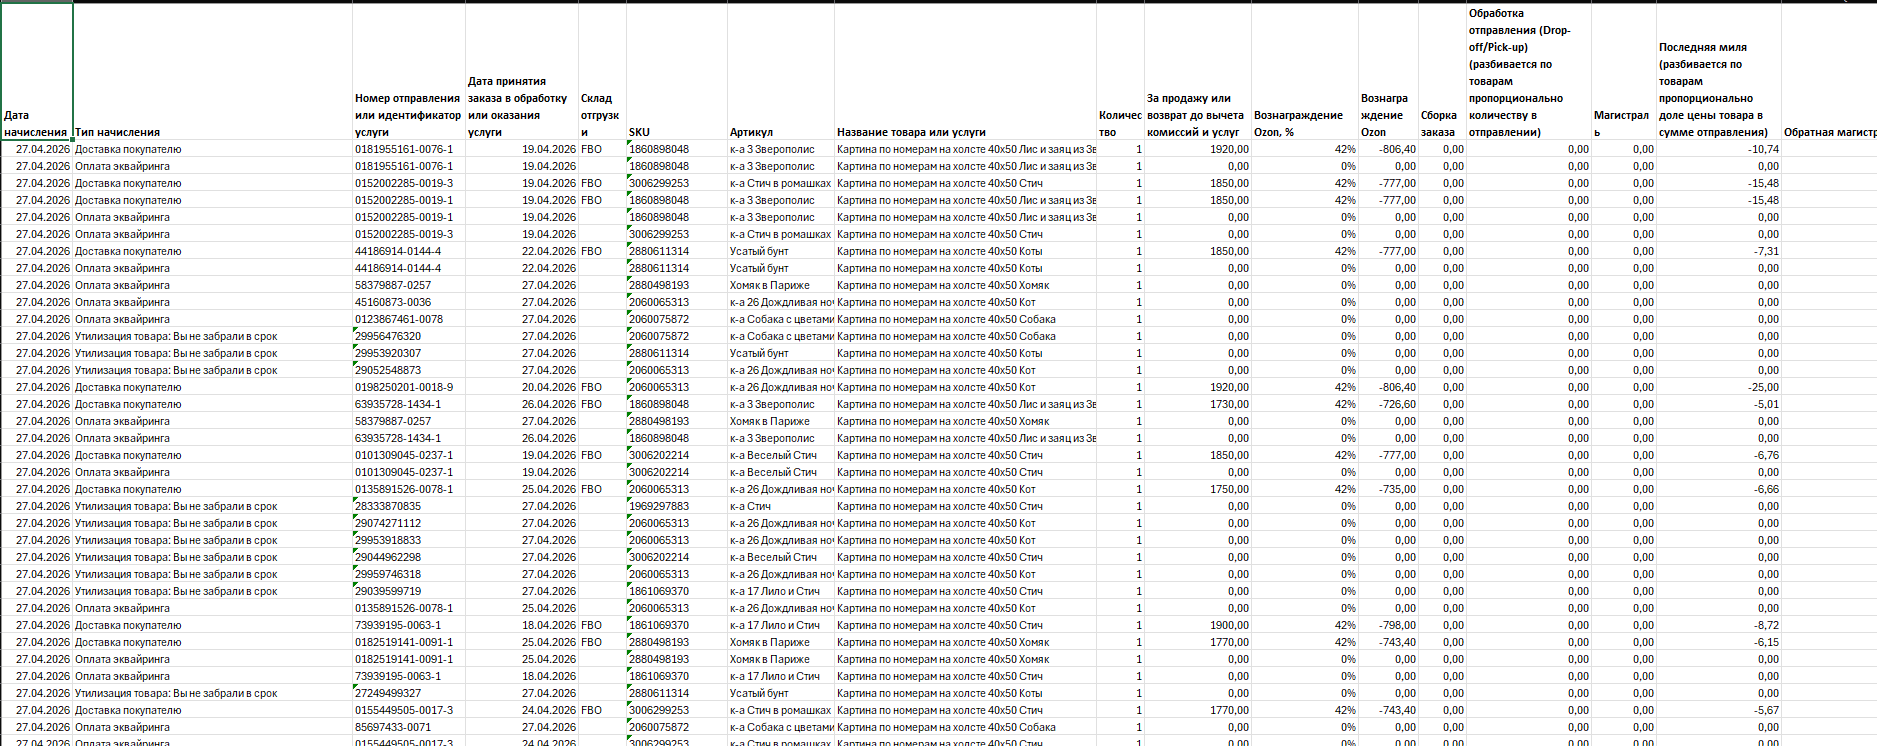
\includegraphics[width=1\textwidth]{../image/screen.png}
    \caption{Пример отчета, выдаваемый маркетплейсом.}
    \label{fig:example01}
\end{figure}

Маркетплейсы дают продавцам два основных варианта доступа к информации: через API платформы и через ручную выгрузку отчетов в форматах csv/xlsx из личного кабинета пользователя. Рассмотрим каждый из них.

\subsection{API отчеты}

API – это набор определенных правил, протоколов и инструментов, которые позволяют одному программному приложению взаимодействовать с другим ~\cite{usingAPI}.
 
С помощью этого инструмента можно получать доступ к данным в реальном моменте времени, управлять приложением по четко сформированным правилам, а также контролировать большие объёмы данных.

Для настройки интеграции по API с маркетплейсами требуется специальный токен, который создается в личном кабинете пользователя.

Из минусов важно упомянуть, что если токеном завладеет злоумышленник, то он получит полный доступ к личному кабинету, сможет изменять любые данные, поэтому возникает вопрос безопасности такой системы~\cite{usingAPI}. 

Помимо этого, у ключей есть срок годности и лимиты запросов, следовательно сами токены нужно обновлять. Так же для создания такой системы потребуется надежная ауте ия пользователя для защиты ключа от посторонних, база данных для хранения информация кабинета и о ключах, а также знания работы с API конкретного маркетплейса, что усложняет разработку~\cite{usingAPI}. 

Но метод получения данных по API является наиболее предпочтительным для разработки веб приложения и автоматизации системы, получаемые данные являются самыми актуальными, которые может предоставить маркетплейс, а их доступность выходит на совершенно новый уровень.

\subsection{Файловые отчеты}
Отчеты о продажах, поступлениях и многом другом предоставляют маркетплейсы, вся информация на момент скачивания отчета является актуальной на сегодняшний день с малейшими погрешностями. Данный подход обладает ключевыми преимуществами, по сравнению с API:

\begin{itemize}
    \item Простота реализации – Такая система не требует обязательной аутентификации пользователя, создания личных токенов и их настройки, использования базы данных для хранения самих токенов, а также сложной логики их обработки. Вся логика сосредоточена на парсинге данных и их последующей обработки для структуризации.
    \item Безопасность – Исключение рисков утечек информации, связанные с хранением и передачей токенов доступа API, так как обработка данных происходит на стороне клиента.
\end{itemize}

\begin{table}[H]
\caption{Сравнение Rest API отчетов и обычных отчетов}
\begin{tabular}{|p{5cm}|p{4cm}|p{4cm}|}
\hline
Критерии & Rest API отчеты & Отчеты \\ \hline
Актуальность данных & Реальное время & На день формирования отчета \\ \hline
Сложность реализации & Высокая & Средняя \\ \hline
Требования безопасности & Высокие & Минимальные \\ \hline
Зависимость от платформы & Высокая & Низкая \\ \hline
Необходимость серверной части & Обязательна & Не обязательна \\ \hline
Автоматизация системы & Наивысшая & Минимальная \\ \hline
\end{tabular}
\end{table}

Для целей данной работы выбран подход с использованием отчётов, получаемых через API токены, так как он позволяет автоматизировать систему, получать самые актуальные данные и контролировать их форматирование. Данный подход обеспечивает необходимый баланс между функциональностью, безопасностью и сложностью реализации.

\section{Использование API}
Решение о выборе архитектурного подхода к интеграции с API является ключевым этапом при создании системы автоматизированного сбора и обработки данных маркетплейса. От правильности этого выбора будет зависеть надежность получения данных, стабильность работы приложения и возможности его дальнейшего масштабирования~\cite{ozonapiAsync}.

В отличие от традиционной веб-разработки, где основное внимание уделяется выбору языка программирования, при работе с API торговых платформ на первый план выходят следующие критерии:

\begin{enumerate}
    \item Протоколы взаимодействия: современные маркетплейсы, используют REST API как основной стандарт обмена данными. REST работает поверх протокола HTTP и использует стандартные методы запросов (GET, POST, PUT, DELETE), что обеспечивает универсальность и простоту интеграции~\cite{ozonapiAsync}.
    \item Форматы обмена данными: API маркетплейсов, используют JSON (JavaScript Object Notation) как основной формат передачи данных. JSON стал отраслевым стандартом благодаря своей легкости, читаемости и совместимости с любыми языками программирования~\cite{ozonapiAsync}.
    \item Аутентификация и безопасность: Работа с API маркетплейсов требует надежной системы аутентификации. Ozon API использует двухкомпонентную систему: Client-ID и API-ключ, которые передаются в заголовках каждого запроса. Это обеспечивает защиту от несанкционированного доступа и позволяет идентифицировать каждое обращение к серверу~\cite{ozonapiAsync}.
    \item Асинхронность операций: Важной особенностью API Ozon является асинхронная модель формирования отчетов. При запросе большого объема данных сервер не возвращает их мгновенно, а создает задачу и предоставляет уникальный идентификатор, по которому впоследствии можно получить готовый отчет. Такой подход позволяет эффективно распределять серверные ресурсы и обрабатывать запросы любого объема~\cite{ozonapiAsync}.
    \item Кроссплатформенность: API-интеграция не привязана к конкретному языку программирования или операционной системе. Любое приложение, способное отправлять HTTP-запросы и обрабатывать JSON-ответы, может взаимодействовать с API Ozon. Это обеспечивает свободу выбора технологий на стороне клиента и возможность поэтапного развития системы~\cite{ozonapiAsync}.
\end{enumerate}

Таким образом, при проектировании системы сбора отчетности выбор делается не столько в пользу конкретного языка программирования, сколько в пользу понимания API маркетплейса, форматов данных и моделей взаимодействия с сервером маркетплейса~\cite{retailcrmOzon}.

\section{Аутентификация и авторизация пользователей в веб-приложениях}

При разработке многопользовательских веб-приложений, работающих с конфиденциальными коммерческими данными, критически важным становится разграничение доступа между пользователями~\cite{authBasics}. Для этого применяются два взаимосвязанных процесса: аутентификация и авторизация. Несмотря на схожесть терминов, они решают разные задачи.

Аутентификация – это процесс проверки подлинности пользователя, то есть подтверждение того, что пользователь является тем, за кого себя выдаёт. В большинстве веб-приложений аутентификация реализуется через ввод пары «логин (email) – пароль»~\cite{authBasics}. Система сравнивает введённые данные с теми, что хранятся в базе данных, и при совпадении предоставляет пользователю доступ~\cite{bookWebAuth}.

Авторизация – это процесс определения прав доступа аутентифицированного пользователя к определённым ресурсам или функциям системы~\cite{authBasics}. Если аутентификация отвечает на вопрос «кто пользователь?», то авторизация – «что пользователь может делать?». В рамках данной работы авторизация реализована на уровне маршрутов: неавторизованный пользователь не может получить доступ к страницам аналитики, даже если введёт их URL вручную~\cite{bookNextjs}.

\subsection{Методы хранения паролей: хеширование и шифрование}

Одной из главных угроз безопасности веб-приложений является хищение и взлом баз данных с учётными записями пользователей~\cite{owaspPasswords}. Хранение паролей в открытом виде недопустимо, так как при утечке базы данных злоумышленник получает полный доступ к аккаунтам всех пользователей. Для защиты паролей применяются два основных подхода: шифрование и хеширование~\cite{bookCryptography}.

Шифрование – это двусторонний процесс преобразования данных с использованием ключа. Зашифрованные данные можно расшифровать обратно в исходный текст при наличии правильного ключа. Шифрование применяется для передачи данных по сети (например, HTTPS/TLS) или для хранения данных, которые могут понадобиться в исходном виде. Однако для хранения паролей шифрование не подходит, так как злоумышленник, получивший доступ к базе данных и ключу шифрования, сможет расшифровать все пароли.

Хеширование – это одностороннее преобразование данных в строку фиксированной длины (хеш, или хеш-сумму). Главное свойство хеширования – необратимость: по полученному хешу невозможно восстановить исходный пароль~\cite{bcryptDocs}. При регистрации пользователя система вычисляет хеш пароля и сохраняет именно его. При последующем входе система повторно вычисляет хеш от введённого пароля и сравнивает его с сохранённым хешем. Если хеши совпадают – пароль введён верно. Сам исходный пароль при этом нигде не хранится.

Однако простые хеш-функции уязвимы для атак по словарям и радужным таблицам. Злоумышленник может предварительно вычислить хеши для всех распространённых паролей и быстро найти соответствие. Для защиты от таких атак применяются два механизма: соль и адаптивное хеширование~\cite{bcryptDocs}.

Модификатор входа хеш-функции – это случайная строка, которая добавляется к паролю перед хешированием. Соль генерируется индивидуально для каждого пользователя и сохраняется вместе с хешем~\cite{owaspPasswords}. Даже если два пользователя имеют одинаковый пароль, благодаря разным солям их хеши будут различаться. Это делает атаки по радужным таблицам неэффективными.

Адаптивное хеширование – это метод, при котором функция хеширования выполняется многократно (обычно тысячи или десятки тысяч раз), что значительно увеличивает время вычисления хеша. Для пользователя это замедление незаметно (доли секунды), но для злоумышленника, перебирающего миллионы паролей, такое замедление делает атаку практически невозможной. В данной работе используется библиотека bcrypt, которая реализует адаптивное хеширование с автоматическим добавлением модификатора входа хеш-функции~\cite{bcryptDocs}.

\subsection{Управление сессиями: JWT и HTTP-only cookies}

После успешной аутентификации приложению необходимо запомнить, что пользователь вошёл в систему, чтобы не требовать повторного ввода пароля при каждом переходе между страницами. Для этого используются механизмы управления сессиями~\cite{jwtIntro}. В современных веб-приложениях наиболее распространены два подхода: серверные сессии (с хранением состояния на сервере) и токен-ориентированная аутентификация (клиентские токены). В данной работе реализован второй подход с использованием JWT~\cite{bookJWT}.

JWT (JSON Web Token) – это открытый стандарт (RFC 7519) для создания компактных и самодостаточных токенов, передающих информацию между сторонами в виде JSON-объекта~\cite{jwtIntro}. JWT состоит из трёх частей, разделённых точками:
\begin{itemize}
    \item Header (заголовок) – содержит информацию о типе токена и алгоритме подписи (например, HS256);
    \item Payload (полезная нагрузка) – содержит утверждения о пользователе: идентификатор, email, время создания и время истечения токена;
    \item Signature (подпись) – создаётся путём шифрования заголовка и полезной нагрузки с использованием секретного ключа. Подпись гарантирует, что токен не был изменён после создания~\cite{jwtIntro}.
\end{itemize}

Преимущества JWT:

\begin{enumerate}
    \item Самодостаточность – токен содержит всю необходимую информацию о пользователе, что снижает нагрузку на сервер~\cite{jwtIntro};
    \item Масштабируемость – серверу не нужно хранить состояние сессии, что упрощает горизонтальное масштабирование~\cite{bookJWT};
    \item Механизм истечения – токены автоматически становятся недействительными по истечении заданного времени~\cite{jwtIntro}.
\end{enumerate}

Однако JWT-токен необходимо безопасно хранить на клиенте. Наиболее распространённый способ – использование HTTP-only cookies~\cite{cookieSecurity}.

HTTP-only cookies – это файлы cookie, которые имеют флаг HttpOnly. Этот флаг запрещает доступ к cookie из клиентского JavaScript-кода, что эффективно защищает токен от XSS-атак (межсайтовый скриптинг)~\cite{owaspXSS}. Даже если злоумышленник внедрит вредоносный скрипт на страницу, он не сможет украсть JWT-токен. Дополнительно устанавливаются флаги Secure (передача только по HTTPS) и SameSite=lax (защита от CSRF-атак)~\cite{cookieSecurity}. В разработанном приложении при успешном входе сервер устанавливает HTTP-only cookie с JWT-токеном, и при каждом последующем запросе браузер автоматически отправляет эту cookie на сервер.

\subsection{Защита маршрутов: proxy (middleware)}

Для предотвращения доступа неавторизованных пользователей к защищённым разделам веб-приложения необходимо проверять наличие валидной сессии при каждом переходе между страницами. В Next.js эта задача решается с помощью механизма middleware (в версии 16 переименован в proxy)~\cite{nextjsMiddleware}.

Proxy-функция выполняется на сервере перед обработкой каждого входящего запроса. Она проверяет наличие и валидность JWT-токена в cookie и принимает решение:

\begin{itemize}
    \item Если пользователь не авторизован и пытается зайти на защищённую страницу (аналитика, дашборд) – происходит перенаправление на страницу входа~\cite{nextjsMiddleware};
    \item Если пользователь авторизован и пытается зайти на страницу входа или регистрации – происходит перенаправление на главную страницу~\cite{nextjsMiddleware}.
\end{itemize}

Такой подход обеспечивает единую точку контроля доступа и исключает необходимость дублировать проверки на каждой странице~\cite{bookNextjs}.



\section{Хранение учётных записей}

Для постоянного хранения зарегистрированных пользователей в веб-приложении используется база данных SQLite. Это легковесная встраиваемая система управления базами данных, которая не требует отдельного серверного процесса и хранит все данные в одном файле (users.db). Таблица пользователей содержит следующие поля:

\begin{itemize}
\item id – уникальный идентификатор пользователя (формат UUID);
\item email – адрес электронной почты (используется в качестве логина);
\item password\_hash – хеш пароля, сгенерированный bcrypt;
\item created\_at – дата и время регистрации.
\end{itemize}

Выбор SQLite обусловлен простотой развёртывания, отсутствием необходимости в настройке отдельного сервера баз данных и достаточной производительностью для малого и среднего количества пользователей и данных.

\section{Используемые технологии в проекте}
В разработанном веб-приложении для реализации аутентификации и авторизации применяются следующие технологии:

\begin{table}[H]
\caption{Технологии и компоненты системы аутентификации}
\begin{tabular}{|l|l|l|}
\hline
Компонент & Технология & Назначение \\ \hline
Хеширование паролей & bcrypt & Адаптивное хеширование \\ \hline
Токены сессий & JWT & Создание токенов \\ \hline
Хранение токенов & HTTP-only cookies & Хранение токенов, защита от XSS \\ \hline
Защита маршрутов & Next.js proxy & Проверка авторизации \\ \hline
База данных & SQLite & Хранение учётных записей \\ \hline
Язык реализации & TypeScript & Типизированная надстройка \\ \hline
\end{tabular}
\end{table}

Таким образом, выбранный комплекс технологий обеспечивает надёжную защиту пользовательских данных, удобство использования и масштабируемость системы.

\begin{table}[H]
\caption{Технические инструменты разработки сайта}
\begin{tabular}{|l|l|}
\hline
Назначение & Технология \\ \hline
Разметка страниц & HTML5 \\ \hline
Стилизация и адаптивность & CSS + Tailwind CSS \\ \hline
Язык программирования & TypeScript \\ \hline
Фреймворк & Next.js 16 (App Router) \\ \hline
API-запросы & Fetch API / HTTPS \\ \hline
Авторизация & JWT + bcrypt + HTTP-only cookies \\ \hline
База данных пользователей & SQLite \\ \hline
Работа с Excel/CSV & XLSX \\ \hline
Защита маршрутов & Proxy Next.js \\ \hline
\end{tabular}
\end{table}

